\chapter[\FermiLAT and the $\gamma$-Ray Sky]{\FermiLAT and the $\gamma$-Ray Sky}
In this chapter I provide an overview of the design and analysis abilities of the Large Area Telescope on board the \Fermi Gamma Ray Space Telescope (otherwise known as \FermiLAT). \FermiLAT is a whole-sky imaging gamma-ray telescope currently in low-Earth orbit which is capable of detecting photons from about 10 MeV to more than 1 TeV in energy. For a more in-depth description of the LAT design, the \FermiLAT collaboration provides technical paper \cite{collaboration_large_2009}. 

\section{History}
The field of gamma ray astronomy begins in earnest with a paper by Morrison in 1958 \cite{morrison_gamma-ray_1958} which lays out the motivation for making astronomical observations at high energies. The crux of Morrison's argument is that visible light from high-energy processes is only created indirectly- the nuclear reactions that power stars, for example, are screened by huge amounts of stellar medium. High-energy charged particles are directly produced by energetic processes, but they are deflected by magnetic fields, obscuring their origin. Gamma rays, on the other hand, are produced directly in high-energy processes and are unaffected by magnetic fields, therefore providing a window into new physical processes. 

Morrison's ideas were influential in the creation of a number of balloon-based gamma ray instruments, as well as the space-based telescopes {\textit {Agile}} and EGRET. A proposal for the telescope that would eventually become \Fermi-LAT was first put together in 1994. During the next 14 years, an international collaboration of scientists and engineers, primarily from the United States, Italy, Japan, and Sweden worked together to build \Fermi. On June 11, 2008, the \Fermi Gamma Ray Space Telescope was successfully launched into low-Earth orbit aboard a Delta II Heavy launch vehicle. In its ten years in orbit, \Fermi has successfully measured the angular positions, energies, and arrival times of over 1 billion photons. 

\section{Design}
The design of \FermiLAT is informed by the fact that gamma rays cannot be focused or reflected in the same manner as visible light, as their wavelength is far smaller than typical atomic spacing. Instead of measuring the gamma rays directly, \FermiLAT causes incident gamma rays to pair-convert into electrons and positrons whose momenta are then measured. Pair-conversion is an important background rejection feature, as only e+/e- pairs that originate from within the LAT are eligible gamma-ray candidates. The measurement of the e+/e- momenta takes place in two stages- directional information is reconstructed from hits in silicon strip sensors in the tracker, while energies are measured via detection of scintillation light in the calorimeter.

\subsection{Tracker}
There are 16 individual tracker towers on the LAT, arranged in a 4x4 grid. Each tower has 18 double layers of orthogonally-oriented silicon strip detectors. 16 layers of a high-Z material (tungsten foil) are placed in front of each of the first 16 pairs of silicon strip detectors, providing a location where the gamma rays can pair-convert into an electron and positron. Electron/hole pairs are created in the silicon detectors as the pair-produced electrons and positrons pass through them, which are then read out by electronics. The recorded positions of the electron/positron pair are recorded at each subsequent tracker layer, and a track reconstruction algorithm (generally based on a Kalman filter) is used to find the path of the e+ and e-.

As the e+/e- pairs traverse the tracker layers, they undergo multiple scattering (especially by the tungsten foils), which limits the angular resolution available. On the other hand, the probability of a gamma ray conversion event is proportional to the thickness of the tungsten, so a compromise between two competing goals (good angular resolution and high conversion efficiency) must be reached. In the LAT, the compromise made was to separate the tungsten into two groups: the first 12 layers are relatively thin (the "front") while the last 4 layers ("back") are approximately 6 times thicker. The total number of radiation lengths is approximately equal in the "front" and "back" segments, though the front-converting photons have somewhat better angular resolution, by roughly a factor of two.
The angular resolution of \FermiLAT for "front"- and "back"- converting photons is represented in Figure X by the 68\% containment radius. Notably, the resolution improves dramatically as the energy of the incident photon increases- this is a consequence of the fact that a typical multiple scattering angle is inversely proportional to the energy of a particle.

\subsection{Calorimeter}
Below each tracker tower lies a calorimeter module containing 96 scintillating thallium-doped cesium iodide crystals, read out by PIN photodiodes. The crystals are oriented in 8 rows of 12 crystals in a hodoscopic array, yielding a total calorimeter depth of 8.6 radiation lengths. As the primary high-energy electrons and positrons from the tracker encounter the dense calorimeter medium, they radiate secondary photons which can themselves pair-produce electron-positron pairs. The process continues until the energy of the gamma rays in the resulting electromagnetic shower falls below the rest energy of an electron, yielding a shower shape that is sensitive to the total energy of the primary electron or positron. 
With its segmented array, the LAT calorimeter modules are capable of measuring both the energy and shape of the electromagnetic shower. The reconstructed energy is simply the sum of all the collected energy in the scintillators, subject to corrections (estimated from Monte Carlo studies) for showers that are large enough to escape the detector volume. The eigenvectors of the shower shape are then computed and used to guess a preliminary track direction to seed the track reconstruction algorithm.

\subsection{Anticoincidence Detector}
Surrounding the tracker and calorimeter is a segmented anti-coincidence detector composed of scintillating plastic, whose purpose is the rejection of charged particle backgrounds from cosmic rays. The material of the ACD is chosen to be low-Z so as to not absorb any gamma-rays, and to not provide a location for incident protons to generate pions (which would generate a substantial background by subsequent decay to two gamma rays). 
Events are vetoed only if the ACD triggers at a position consistent with reconstructed track, which prevents spurious vetos from 'backsplash'- an effect that occurs when the EM shower in the calorimeter causes the emission of secondary particles that strike the ACD. By segmenting the ACD into 89 tiles, these self-veto events are present for less than 20\% of the photons at 300 GeV, compared to ~50\% at 10 GeV for the non-segmented EGRET.

\subsection{Data}
\Fermi most often operates in 'survey mode', during which it scans the entire sky with roughly equal exposure on a time scale of ~3 hours. However, alternate observing patterns are relatively common, such as when \Fermi reorients itself to observe the potential afterglow of a LIGO event, or points towards a flaring blazar for an extened period. Other interruptions to regular data collection include the times \Fermi traverses the South Atlantic Anomaly (during which the event rate becomes extremely high), and the handful of orbits during which \Fermi has faced the Earth in order to detect terrestrial gamma-ray flashes from lightning.

Data collected by \FermiLAT is downloaded via radio link in ~1.5 Gb intervals approximately every 3 hours to NASA's Goddard Space Flight Center, and sent on to SLAC National Accelerator Laboratory for processing to reconstruct photon properties and reject background signals. Photons detected by \FermiLAT are typically available for download from the GSFC within 8 hours of their arrival.

\section{$\gamma$-Ray Sky}
A typical \FermiLAT gamma ray has an energy in the GeV range. An approximate measure for the corresponding temperature of such a photon is given by E/k= $10^13$ K, for comparison, the temperature at the center of the Sun is approximately $10^7$ K. Therefore high-energy gamma rays are generally produced by a handful of non-thermal processes. Relativistic charged particles can emit synchrotron radiation in the presence of magnetic fields, and bremsstrahlung radiation upon interactions with matter. Neutral pions decay to two gamma rays, and excited nuclei can de-excite via the emission of a gamma ray. In Chapter 6, I will discuss the potential for dark matter to annihilate to final states that include gamma rays.
With this in mind, it is not surprising that the gamma-ray sky looks rather different from the sky in the optical band- see Figure \ref{fig:fermi5year}. A number of features are readily apparent from the whole-sky image:

\begin{figure}
\begin{center}
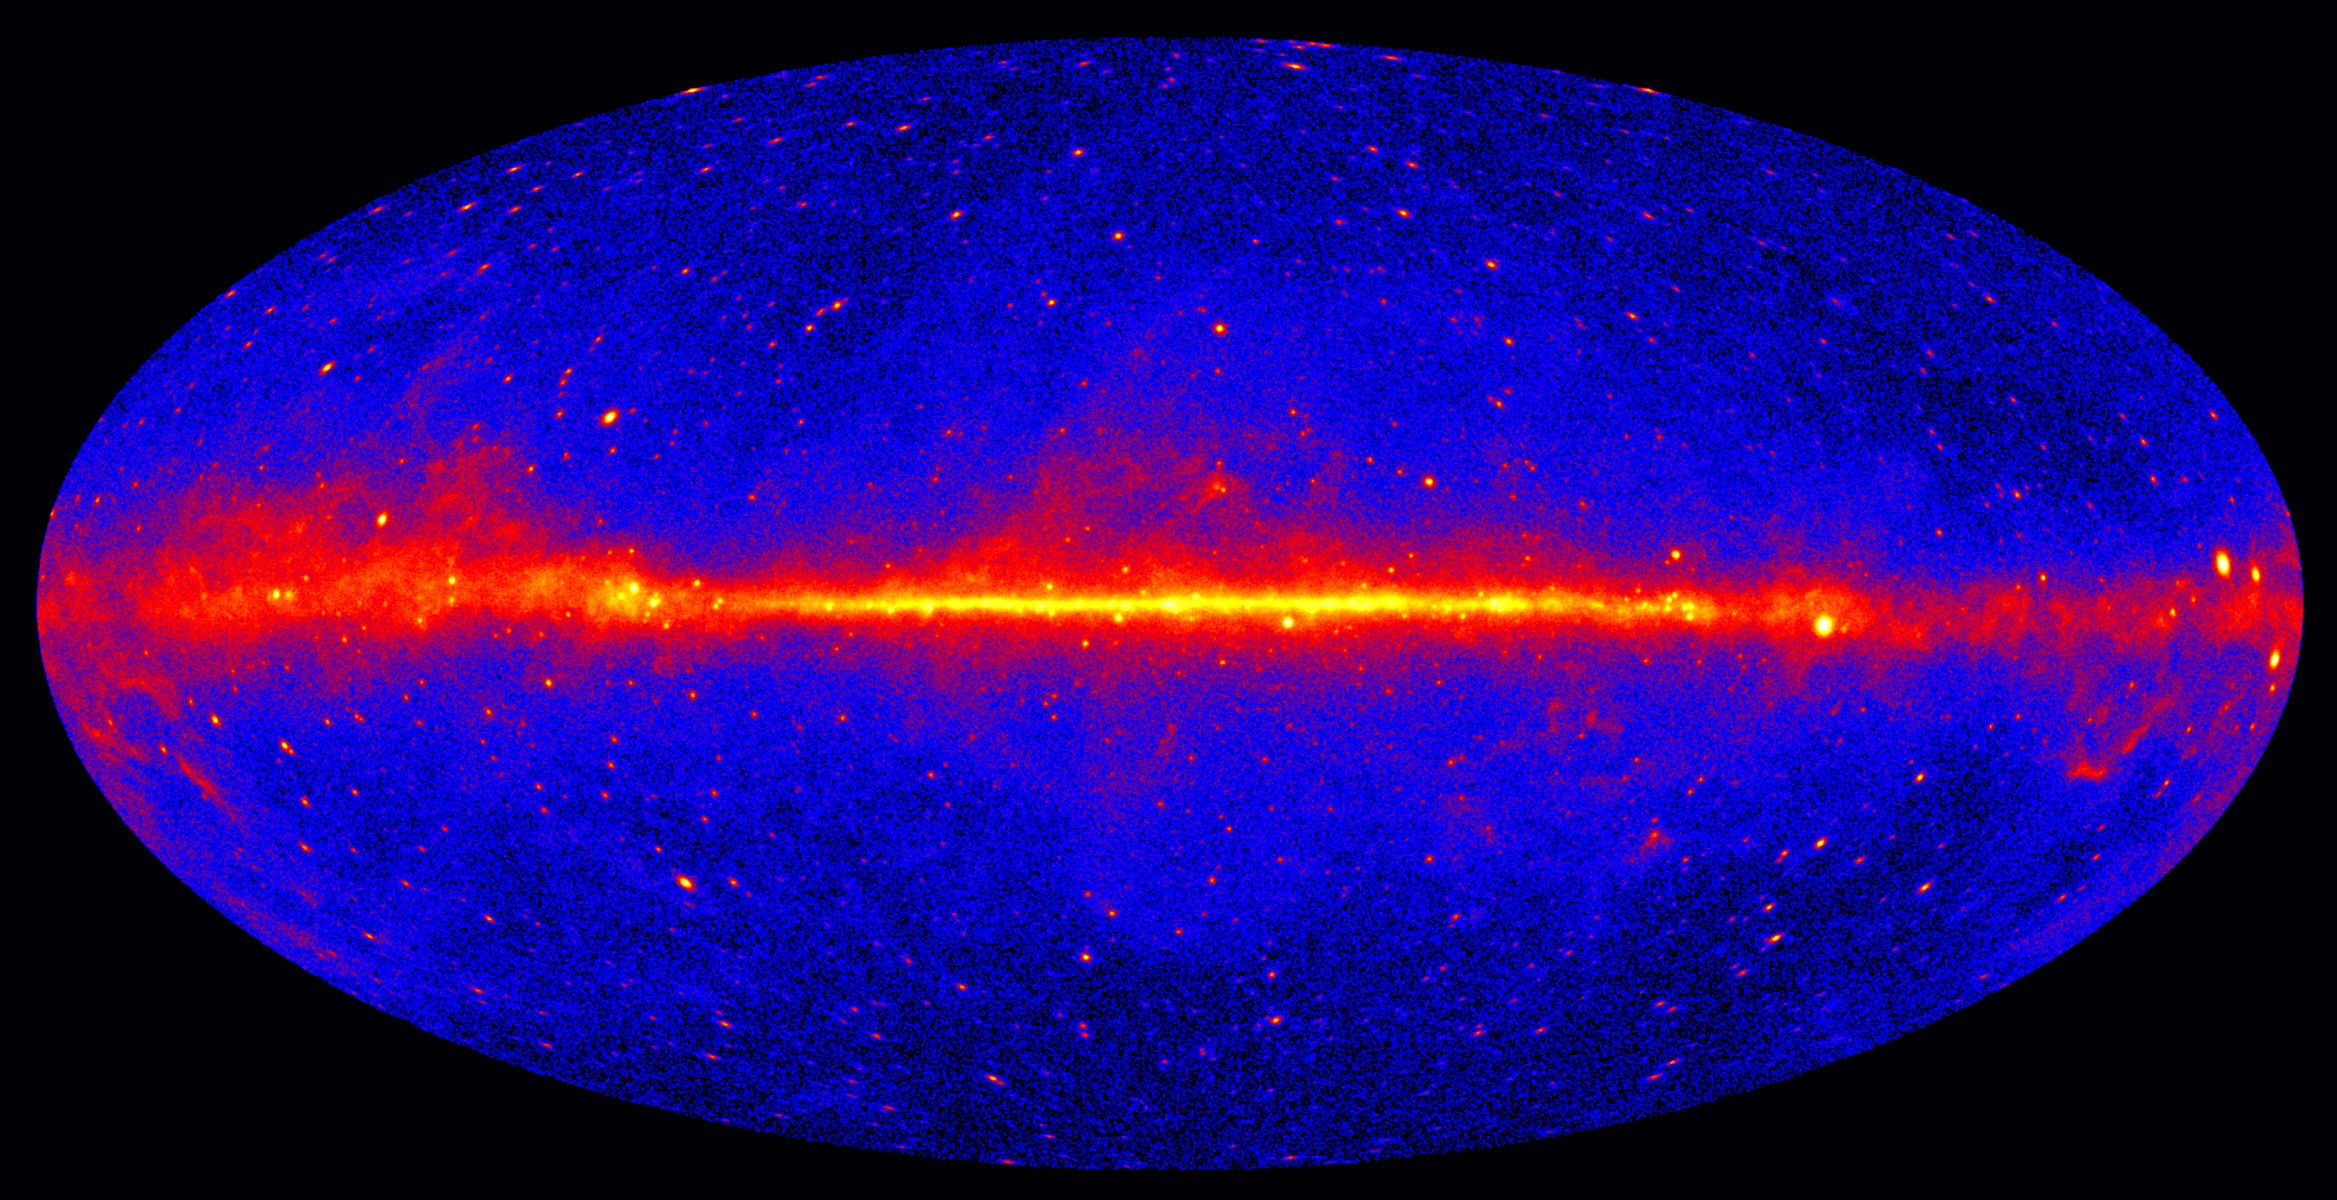
\includegraphics[width=0.9\columnwidth]{figures/Fermi_5_year.jpg}
\caption{
\label{fig:fermi5year}
The Fermi sky in Galactic coordinates using an Aitoff projection.
Color corresponds to the integrated flux above 1 GeV over 5 years.
The Galactic plane features prominently across the center of the image, while numerous point sources are seen across the entire sky.
{\it Image credit: NASA/DOE/\Fermi-LAT Collaboration}
}
\end{center}
\end{figure}
\subsection{Diffuse emission}
Much of the sky's gamma ray emission is in the Galactic plane, and is due to highly energetic charged particles interacting with the interstellar medium. These interaction generally produce neutral pions which then decay to two gamma rays, the energy of which depends on the energy of the initial cosmic ray. 
The origin of high-energy cosmic rays was a mystery for some time, as 2nd-order \Fermi acceleration seemed insufficient to produce particles with energy >10 GeV. A number of authors in the 1970s, however, discovered that collisionless shock boundary of supernova remnants could sufficiently energize charged particles. At the shock boundary, the magnetic field is nearly discontinuous, and 1st order \Fermi acceleration is sufficient to produce charged particles in the many-GeV energy range.
Models of the galactic diffuse emission are generated by the \FermiLAT collaboration by fitting templates of interstellar emission at several wavelengths to observed regions of the $\gamma$-ray sky \cite{acero_development_2016}.
 
Some diffuse emission extends beyond the Galactic plane, and appears to be isotropic across the sky. Most of this isotropic component is believed to originate from unresolved point sources (see below), though some backgrounds of cosmic rays and improperly reconstructed photons from the Earth limb also contribute.
\subsection{Point Sources}

\subsubsection{Blazars}
Most large galaxies contain a rapidly rotating supermassive black hole at their center, some of which actively accrete material. These so-called "active galaxies" possess two main features- a thermal accretion disk, and a relativistic jet aligned along the black hole's rotation axis. When the Earth lies in the direction of a jet axis, the active galaxy is called a blazar and is a bright sources of gamma rays.

The highly relativistic particles in the jet are believed to derive their power directly from the supermassive black hole. Via the Blandford-Znajek process \cite{blandford_znajek_1977}, magnetic fields from the accretion disk which reach inside the black hole's ergosphere can extract rotational energy from the black hole, and the subsequent rotation of the magnetic field causes charged particles to be accelerated to high speeds along the jets. These relativistic particles can then emit gamma rays via synchrotron radiation, bremsstrahlung, or inverse Compton scattering. 
\subsubsection{Pulsars}
Rapidly rotating neutron stars known as pulsars are one of the most numerous point sources in the gamma-ray sky. Surrounded by extraordinarily powerful and rapidly rotating magnetic fields, pulsars emit gamma rays as electrons stripped from their surface emit synchrotron radiation. A small number of pulsars have periods smaller than 1 second, and are referred to as millisecond pulsars; a novel and unresolved population of millisecond pulsars may exist near the Galactic center and contribute to the $\gamma$-ray excess that has been observed there by a number of authors (e.g. \cite{bhakta_searching_2017}).
\subsubsection{Galactic Center}
	The brightest source in the gamma-ray sky by far is the Galactic center, containing the supermassive black hole at the center of the Milky Way located at Sag A*. A number of models have been proposed to explain the gamma-ray emission at Sag A*, generally involving charged particles interacting with the surrounding medium \cite{van_eldik_gamma_2015}. These particles may be injected into the region by tidal disruption of stars by Sag A*. As discussed in Chapter 6, some DM models predict annihilation to occur in the region surrounding Sag A* as well, which may lead to gamma-ray emission.

\section{Analysis Tools}\label{sec:analysisTools}

\FermiLAT data and LAT-specific analysis tools are publicly available for download from the \Fermi Science Support Center at NASA's Goddard Space Flight Center \footnote{{\tt https://fermi.gsfc.nasa.gov/ssc/}}. 
Processing \FermiLAT data for analysis begins by removing photons (via the tool {\tt gtselect}) that are incident from near the Earth limb, as these mostly originate from cosmic ray interactions with the atmosphere. For a typical analysis, the photons are then binned (with the use of the tool {\tt gtbin}) in angular position and energy. The LAT effective area is convolved (by use of the tool {\tt gtltcube}) with its pointing history over the time period considered to produce an exposure map binned in energy and angular position. 
Typical \FermiLAT analyses make use of maximum likelihood techniques to test differing hypotheses (spectral features, location, etc) about sources in question. The process begins by defining a model of the region of interest (ROI). A model is composed of a list of sources, each of which is defined by its spectral shape, position on the sky, and spatial appearance. With a model and the exposure map, the expected number of photons $\mu_i$ in each bin $i$ can be computed and compared to the actual counts $n_i$. The value of the likelihood for the model is then given by the product of Poisson factors over the number of bins $N$:
\begin{equation}
\mathcal{L} = \prod_{i=1}^{N} \frac{\mu_i^{n_i}}{n_i!}e^{-\mu_i}
\end{equation}
By varying the parameters in the model, the likelihood can be maximized. In cases with sufficient statistics and where the parameters satisfy Wilks criteria, the value of the delta log-likelihood between two hypotheses follows a $\chi^2$ distribution \cite{wilks_1938}. If this is the case, the significance of the varied parameter can be determined; if this is not the case, the significance can be determined through a Monte Carlo study.

The \FermiLAT collaboration has successfully used these techniques to compile several catalogs of gamma-ray sources. The most current catalog is the Third \Fermi Source Catalog \cite{collaboration_fermi_2015} (hereafter referred to as 3FGL). The 3FGL composed of 3033 sources, of which a majority (3008) of which are point sources and 25 of which are modeled as extended. A large fraction of the sources are pulsars or active galaxies, but a sizable component (1010) are unassociated with any known sources. I make use of the 3FGL in Chapter 4 to identify potential PBH candidates, and to place limits on their presence.